\chapter{Prostheses and control} \label{prostheses}

A prostheses is many things, for some it is to give visual sense of having both arms fingers or legs, where others has some functionality build in.
There are many types of prosthesis, here is a short description of the different types prosthesis that is on the market right now.

\paragraph{Aesthetics prostheses}
This is a prosthesis that is mainly used for the user of prosthesis can, feel as part of the society without having to answer, every curious gaze from bystanders. Aesthetics is often seen as a passive device, but supports the user so the body weight is more uniform\cite{aesthetic}.  
\begin{figure}[H]
    \centering
    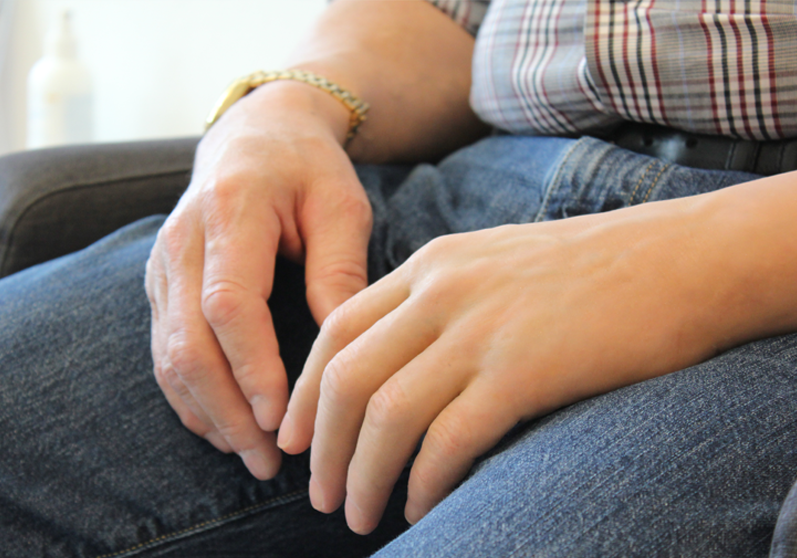
\includegraphics[width=10cm,height=7cm]{Figures/Contextual_figures/ProsthesesPics/aestikarm.png}
    \caption{aesthetic arm prostheses from Shava\cite{aesthetic}.}
    \label{fig:aesthetic}
\end{figure}
\paragraph{Mechanical prostheses}
A mechanical arm is made depending on the users amputation level,some are operated with the elbow joint and some with the wrist and for high level amputees such as shoulder disarticulation, moves the arm in position, with the other hand, if for instance a user wants to lift a box, the user manipulates the arm whit the other hand, so it can grasp the box in collaboration, with the able hand. 
\begin{figure}[H]
    \centering
    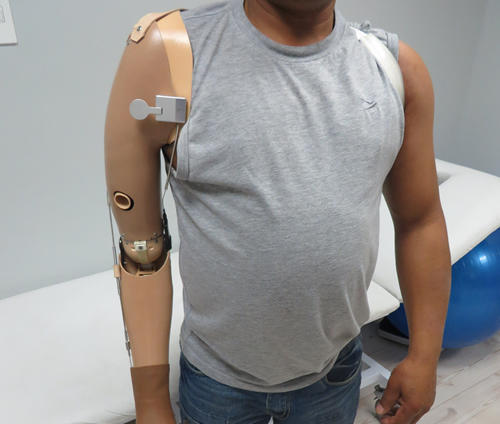
\includegraphics[width=10cm,height=7cm]{Figures/Contextual_figures/ProsthesesPics/above-elbow-prosthesis-500x500.jpg}
    \caption{A mechanical prostheses operated by wire\cite{AEP}.}
    \label{fig:AEP}
\end{figure}
\subsection*{Electrical prostheses}
As the word implies, these are electric, meaning that they have a motor or actuators to move the joints of the prostheses and can be used with different controllers and control systems. These prosthesis are also the most expensive and advanced to use. Since the goal of the project is to provide as much support for the individual user, the mechanical prostheses is superior. Some of the electrical prostheses already on the market is seen below.
\begin{figure}[H]
    \centering
    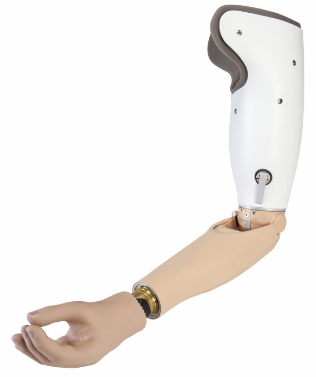
\includegraphics[width=6cm,height=6cm]{Figures/Contextual_figures/ProsthesesPics/dynamixarm.PNG}
    \caption{An Above elbow prosthesis with DynamicArm from Ottobock\cite{OttobockAB} }
    \label{fig:DynaArm}
\end{figure}
DynamicArm is a robotic prosthesis solution from Ottobock, this for a person whom has had an amputation above the elbow joint. DynamicArm provides the user with the ability to flex the elbow joint\cite{OttobockAB}. The prosthesis can be used in combination with the Michelangelo hand which can rotate the wrist and due to different grips\cite{OttobockM}. This is prosthesis used in combination with the Axon-Bus Prosthetic System, this bus system delivers a reliable source for data to the prosthesis and is safe for the user\cite{OttobockAX}.\\
\subsubsection*{Jaco}
Jaco is a stationary robotic manipulator. It is designed to be attached to a wheelchair operating as a left or right arm.\\
It weighs 5.2 kg, which makes it lightweight and unnoticeable for the wheelchair user. The reach is 90 cm, and it utilises 6 D.O.F's. It comes with a default joystick, that has many features, such as operating each joint of the arm and the fingers. Jaco can also initiate a "drinking mode", where it helps the user lift the cup and rotate the wrist for the user to drink from the cup \cite{JACO}.\\
Here is a picture of how its usually used:
\begin{figure}[H]
    \centering
    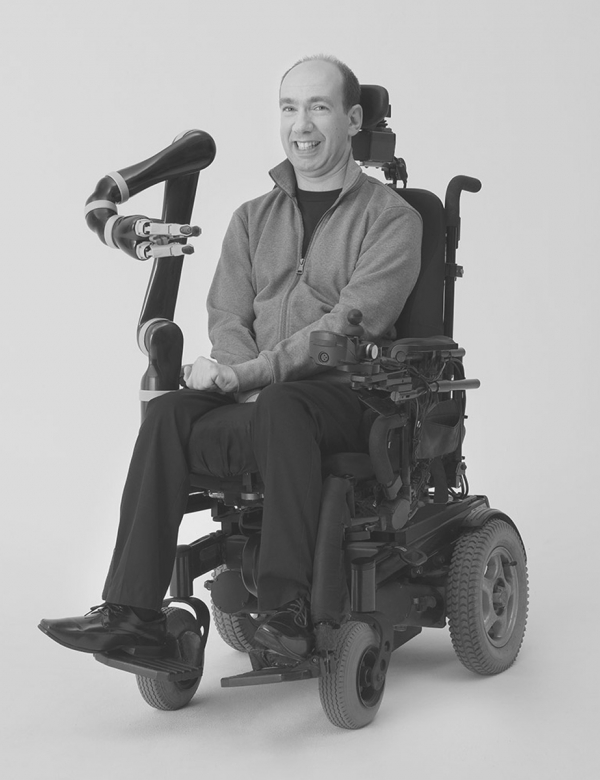
\includegraphics[width=7cm,height=7cm]{Figures/Technical_figures/Sebastien.jpg}
    \caption{Sabastién from Kinova, All rights reserved to Kinova \ref{fig:KinovaPicture} \cite{Kinova}.}
    \label{fig:Sebastién}
\end{figure}
